%%%%%%%%%%%%%%%%%%%%%%%%%%%%%%%%%%
% Beamer presentation
% Created by Nho Gia Hien NGUYEN
% LaSIE, ULR, France
% Inspired from latextemplate.com
%%%%%%%%%%%%%%%%%%%%%%%%%%%%%%%%%%
\documentclass{beamer}

\mode<presentation> {

% Uncomment the theme you want to activate

%\usetheme{default}
%\usetheme{AnnArbor}
%\usetheme{Antibes}
%\usetheme{Bergen}
%\usetheme{Berkeley}
%\usetheme{Berlin}
%\usetheme{Boadilla}
%\usetheme{CambridgeUS}
\usetheme{Copenhagen}
%\usetheme{Darmstadt}
%\usetheme{Dresden}
%\usetheme{Frankfurt}
%\usetheme{Goettingen}
%\usetheme{Hannover}
%\usetheme{Ilmenau}
%\usetheme{JuanLesPins}
%\usetheme{Luebeck}
%\usetheme{Madrid}
%\usetheme{Malmoe}
%\usetheme{Marburg}
%\usetheme{Montpellier}
%\usetheme{PaloAlto}
%\usetheme{Pittsburgh}
%\usetheme{Rochester}
%\usetheme{Singapore}
%\usetheme{Szeged}
%\usetheme{Warsaw}

% Uncomment the color scheme you want to use

%\usecolortheme{albatross}
%\usecolortheme{beaver}
%\usecolortheme{beetle}
%\usecolortheme{crane}
%\usecolortheme{dolphin}
%\usecolortheme{dove}
%\usecolortheme{fly}
%\usecolortheme{lily}
%\usecolortheme{orchid}
%\usecolortheme{rose}
\usecolortheme{seagull}
%\usecolortheme{seahorse}
%\usecolortheme{whale}
%\usecolortheme{wolverine}

%\setbeamertemplate{footline} % To remove the footer line in all slides uncomment this line
%\setbeamertemplate{footline}[page number] % To replace the footer line in all slides with a simple slide count uncomment this line

%\setbeamertemplate{navigation symbols}{} % To remove the navigation symbols from the bottom of all slides uncomment this line
}

% Change font (XeLaTeX only)
%\usefonttheme{professionalfonts} % using non standard fonts for beamer
%\usefonttheme{serif} % default family is serif
%\usepackage{fontspec}
%\setmainfont{Liberation Serif}

\setbeamertemplate{itemize items}[default]
\setbeamertemplate{enumerate items}[default]
\usepackage{animate}
\usepackage{amsmath}
\usepackage{epigraph}
	\setlength\epigraphwidth{9cm}
	\setlength\epigraphrule{0pt}
\usepackage{graphicx} % Allows including images
\usepackage{booktabs} % Allows the use of \toprule, \midrule and \bottomrule in tables
\usepackage{listings} % Insert code to the presentation
\usepackage{fancyvrb}
\usepackage{graphicx,epstopdf}
\usepackage{mwe}
%\usepackage{fontspec}
%\usepackage{lilyglyphs}
\usepackage{color}
\usepackage{xcolor}
\usepackage{datetime}
\usepackage[english]{babel}
\usepackage{blindtext}
\usepackage{tikz}
\usepackage{minted}
\usepackage{multicol} % automatically make multi columns
\usepackage{skak} % chess
\usepackage{harmony} % music note
\usepackage{musixtex} % music score
\usepackage{chemfig} % chemistry
\usepackage[version=3]{mhchem}
\usepackage{logicpuzzle}
%-------------------------
\hypersetup{
	colorlinks,
	allcolors=.,
	urlcolor=blue,
}
%-------------------------
\usetikzlibrary{positioning,backgrounds} 
\usetikzlibrary{matrix}
\usetikzlibrary{lindenmayersystems}
\usetikzlibrary{shapes,arrows}
\usetikzlibrary{mindmap,trees}
% diagram
\usepackage{smartdiagram}
\smartdiagramset{hienElegantStyle/.style={
		module shape=diamond,
		font=\scriptsize,
		module minimum width=1cm,
		module minimum height=1cm,
		text width=1cm
	}
}
%\usepackage{metalogo}
%\usepackage{dtklogos}
\addtobeamertemplate{navigation symbols}{}{%
	\usebeamerfont{footline}%
	\usebeamercolor[fg]{footline}%
	\hspace{1em}%
	\insertframenumber/\inserttotalframenumber
}
%------------ Animation
\pgfdeclarelayer{dome floor}
\pgfdeclarelayer{dome}
\pgfdeclarelayer{dome surface}
\pgfsetlayers{dome floor,main,dome,dome surface}

\def\addcircle#1#2#3#4{%
	\begingroup%
	\pgfmathparse{#1}\let\R=\pgfmathresult
	\pgfmathparse{#2}\let\cx=\pgfmathresult
	\pgfmathparse{#3}\let\cy=\pgfmathresult
	\pgfmathparse{#4}\let\r=\pgfmathresult
	\begin{pgfonlayer}{dome floor}
		\draw [blue!45!black, fill = blue!45, fill opacity = 0.25]
		plot [domain = 0:360, samples = 40, variable = \i] 
		(\cx+\r*cos \i, \cy+\r*sin \i, 0) -- cycle;
	\end{pgfonlayer}
	\begin{pgfonlayer}{dome surface}
		\draw [red!75!black, fill = red!75, fill opacity = 0.25] 
		plot [domain = 0:360, samples = 60, variable = \t] 
		(\cx+\r*cos \t,\cy+\r*sin \t,
		{sqrt(max(\R^2-(\cx+\r*cos(\t))^2-(\cy+\r*sin(\t))^2, 0))})
		-- cycle;
	\end{pgfonlayer}
	\endgroup%
}

%-------------------------------------
\lstset{language=[LaTeX]TeX,
	texcsstyle=*\bf\color{blue},
	numbers=left,
	breaklines=true,
	keywordstyle=\color{darkgreen},
	commentstyle=\color{red},
	morekeywords={},
	otherkeywords={$,\{ ,\} , [ , ] },
	frame=leftline,
	tabsize=2,
	backgroundcolor=\color{lightgrey},
	escapeinside=||
}

\tikzset{%
	fancy quotes/.style={
		text width=\fq@width pt,
		align=justify,
		inner sep=1em,
		anchor=north west,
		minimum width=\linewidth,
	},
	fancy quotes width/.initial={.8\linewidth},
	fancy quotes marks/.style={
		scale=8,
		text=white,
		inner sep=0pt,
	},
	fancy quotes opening/.style={
		fancy quotes marks,
	},
	fancy quotes closing/.style={
		fancy quotes marks,
	},
	fancy quotes background/.style={
		show background rectangle,
		inner frame xsep=0pt,
		background rectangle/.style={
			fill=gray!25,
			rounded corners,
		},
	}
}

\newenvironment{fancyquotes}[1][]{%
	\noindent
	\tikzpicture[fancy quotes background]
	\node[fancy quotes opening,anchor=north west] (fq@ul) at (0,0) {``};
	\tikz@scan@one@point\pgfutil@firstofone(fq@ul.east)
	\pgfmathsetmacro{\fq@width}{\linewidth - 2*\pgf@x}
	\node[fancy quotes,#1] (fq@txt) at (fq@ul.north west) \bgroup}
{\egroup;
	\node[overlay,fancy quotes closing,anchor=east] at (fq@txt.south east) {''};
	\endtikzpicture}

% change chemitry font
\makeatletter
\def\CF@node@content{%
	\expandafter\expandafter\expandafter
	\printatom\expandafter\expandafter\expandafter
	{\csname atom@\number\CF@cnt@atomnumber\endcsname}%
	\ensuremath{\CF@node@strut}%
}
\makeatother
\setdoublesep{0.35700 em}  % 'Bond Spacing'
\setatomsep{1.78500 em}    % 'Fixed Length'
\setbondoffset{0.18265 em} % 'Margin Width'
\newcommand{\bondwidth}{0.06642 em} % 'Line Width'
\setbondstyle{line width = \bondwidth}
\renewcommand*{\printatom}[1]{{\sffamily\cf{#1}}}

%%%%%%% ZOOM BOX %%%%
\makeatletter
\newsavebox\zb@x
\newcounter{z@@m}
\usepackage{calc}
\newdimen\B@r\newdimen\P@r
\newdimen\@zw\newdimen\@zh\newdimen\@zd

\newcommand{\zoombox}[2][0]{%
	\leavevmode%
	\sbox\zb@x{#2}%
	\setlength\B@r{1pt*\ratio{\wd\zb@x}{\ht\zb@x+\dp\zb@x}}%
	\setlength\P@r{1pt*\ratio{\paperwidth}{\paperheight}}%
	\ifdim\B@r>\P@r\relax%
	\setlength\@zw{\wd\zb@x}\setlength\@zh{\@zw*\ratio{\paperheight}{\paperwidth}}%
	\setlength\@zd{(\@zh-\ht\zb@x-\dp\zb@x)*\real{0.5}+\dp\zb@x}%
	\setlength\@zh{\@zh-\@zd}%
	\else%
	\setlength\@zh{\ht\zb@x+\dp\zb@x}%
	\setlength\@zw{\@zh*\ratio{\paperwidth}{\paperheight}}%
	\setlength\@zh{\ht\zb@x}\setlength\@zd{\dp\zb@x}%
	\fi%
	\makebox[0pt][l]{\makebox[\wd\zb@x][c]{\makebox[\@zw][l]{%
				\pdfdest name {zbfs\thez@@m} fitr
				width  \@zw\space
				height \@zh\space
				depth  \@zd\space
	}}}%
	\pdfdest name {zb\thez@@m} fitr
	width  \wd\zb@x\space
	height \ht\zb@x\space
	depth  \dp\zb@x\space
	\immediate\pdfannot 
	width  \wd\zb@x\space
	height \ht\zb@x\space
	depth  \dp\zb@x\space
	{%
		/Subtype/Link/H/N
		/Border [0 0 #1 [1 2]]
		/A <<
		/S/JavaScript
		/JS (
		if(typeof(zoomed)=='undefined'||!zoomed){
			var lastView=this.viewState;
			if(app.fs.isFullScreen) this.gotoNamedDest('zbfs\thez@@m');
			else this.gotoNamedDest('zb\thez@@m');
			zoomed=true;
		}else{
			this.viewState=lastView;
			zoomed=false;
		}
		)
		>>
	}%
	\usebox{\zb@x}%
	\stepcounter{z@@m}%
} 
\makeatother
%%%%%%%%%%%%%%%%%%%%

%----------------------------------------------------------------------------------------
%	TITLE PAGE
%----------------------------------------------------------------------------------------

\title[LaTeX guide for novices]{\LaTeX{} beamer guide for novices} % The short title appears at the bottom of every slide, the full title is only on the title page

\author{Hien N.G. Nguyen \and Antoine Falaize \and Antoine Monnier} % Your name
\institute[LaSIE] % Your institution as it will appear on the bottom of every slide, may be shorthand to save space
{
University of La Rochelle \\ % Your institution for the title page
\medskip
\textit{nho.nguyen@univ-lr.fr} % Your email address
}
\date{\currenttime, \today} % Date, can be changed to a custom date

% logo of University
\titlegraphic{\includegraphics[height=1cm]{Figures/LogoLaSIE}\hspace*{0.75cm}~%
	\includegraphics[height=1cm]{Figures/ULR}
}

\begin{document}

\begin{frame}
\titlepage % Print the title page as the first slide
\end{frame}

\begin{frame}
\transfade
\frametitle{Overview} % Table of contents slide, comment this block out to remove it
\tableofcontents % Throughout your presentation, if you choose to use \section{} and \subsection{} commands, these will automatically be printed on this slide as an overview of your presentation
\end{frame}

%----------------------------------------------------------------------------------------
%	PRESENTATION SLIDES
%----------------------------------------------------------------------------------------

%------------------------------------------------
\section{Intro} % Sections can be created in order to organize your presentation into discrete blocks, all sections and subsections are automatically printed in the table of contents as an overview of the talk
%------------------------------------------------

\subsection{Basic information} % A subsection can be created just before a set of slides with a common theme to further break down your presentation into chunks

\begin{frame}
\transfade
\frametitle{Why \LaTeX{}?}
\epigraph{By preparing a manuscript in TEX format, you will be telling a
	computer exactly how the manuscript is to be transformed into pages
	whose typographic quality is comparable to that of the world’s finest
	printers.}{D. E. Knuth}
\begin{itemize}
	\item Multi-platform: Windows, Linux, macOS
	\item Huge community supports: StackExchange, LaSIE!
	\item Elegant math equations $ E = mc^2 $, $ \pi \approx \frac{355}{113} $
	\item Citation and reference in a breeze
	\item Reuse \LaTeX{} everywhere!
\end{itemize}
\end{frame}

%------------------------------------------------
% Reserved for other contents
%------------------------------------------------
\begin{frame}
\transfade
\frametitle{Why not \LaTeX{}?}
\begin{itemize}
\item Brief notes, shopping list...
\item You love clicking mouse
\item You hate coding and I hate people
\item You adore Microsoft Word than anything else
\begin{figure}
\centering
\includegraphics[width=0.5\textwidth]{Figures/clippy}
\end{figure}
\end{itemize}
\end{frame}

%------------------------------------------------
\begin{frame}
\transfade
\frametitle{What is \LaTeX{} really?}
\begin{itemize}
\item \LaTeX{} is a `typesetting system'
\item \TeX{} is originally developped by Donald Knuth; \LaTeX{} is a `extended' version of \TeX{}, developped by Leslie Lamport (Lamport + \TeX{} $ \rightarrow $ \LaTeX{})
\item \LaTeX{} is not WYSIWYG\footnote{What you see is what you get} like Word and Libre Writer \\~
 $ \rightarrow $ we have to compile the \LaTeX{} code (.tex) to have PDF/DVI output.

\end{itemize}
\end{frame}

%------------------------------------------------
\begin{frame}
\frametitle{Prerequisites}
What you need to set up and run \LaTeX{}
\begin{enumerate}
\item A text editor (\href{https://notepad-plus-plus.org/}{Notepad++}, gEdit\footnote{default in Ubuntu}, \href{https://www.vim.org/}{VIM}, \href{https://www.texstudio.org/}{TeXStudio}, \href{http://www.xm1math.net/texmaker/}{TexMaker}...) to write .tex document
\item A \LaTeX{} distribution (\href{https://www.tug.org/texlive/}{TeXLive}, \href{https://miktex.org/}{MikTeX}...)
\item A PDF viewer (Adobe Reader, Sumatra PDF...)
\end{enumerate}
\end{frame}

%------------------DEFINITION--------------------
%\begin{frame}
%\frametitle{Some definitions}
%
%\end{frame}

%------------------------------------------------
\subsection{Document structure}
\begin{frame}[fragile]
\transfade
\frametitle{Basic structure of a \LaTeX{} document}

\textbf{Document class}
\begin{Verbatim}[fontsize=\footnotesize,frame=single]
\documentclass[a4,12pt]{article}
\end{Verbatim}
Define the document format (article, presentation,poster...) and style (font, basic margin...)\\~
\textbf{Preample}
\begin{Verbatim}[fontsize=\footnotesize,frame=single]
\usepackage{graphicx}
\end{Verbatim}
Declare packages which provide specific capacities like inputing figures, code high-lighting, drawing, animation\\~
\textbf{Main content}
\begin{Verbatim}[fontsize=\footnotesize,frame=single]
\begin{document}
Content goes here
\end{document}
\end{Verbatim}

\end{frame}
%------------Document-Examlple--------------------
\begin{frame}[fragile]
\frametitle{An example}
\begin{columns}[T]
\begin{column}{0.5\textwidth}
Try saving the below text as .tex and compile
\begin{Verbatim}[fontsize=\tiny,frame=single]
\documentclass{article}
\title{Bonjour LaSIE}
\date{10 april 2018}
\author{Lucky Luke}
\begin{document}
\maketitle
\pagenumbering{gobble}
\newpage
\pagenumbering{arabic}
\section{Section}
Hello World!
\subsection{Subsection}
Structuring a document is easy!
\end{document}
\end{Verbatim}
\end{column}
\begin{column}{0.5\textwidth}
Output:
\begin{figure}
\scalebox{0.2}{
\includegraphics{Figures/firstdoc.png}
}
\end{figure}
\end{column}
\end{columns}
\end{frame}
%------------------------------------------------
\begin{frame}[fragile]
\transfade
\frametitle{Beamer class}
\begin{itemize}
\item Beamer is a document class allows creating presentation from \LaTeX{}.
\item Theme and color scheme can be changed easily by \verb|\usetheme{}| ($ >20$ themes) and \verb|\usecolortheme{}| ($ >10 $ color schemes). View complete catalogue \href{http://deic.uab.es/~iblanes/beamer_gallery/}{here}.
\item Direct output PDF.
\end{itemize}
\end{frame}
%------------------------------------------------
\begin{frame}[fragile]
\transfade
\frametitle{Basic structure of a Beamer presentation}
\begin{Verbatim}[fontsize=\footnotesize,frame=single]
\documentclass[handout]{beamer}
\end{Verbatim}
Add \verb|handout| if you want a printed version\\~
\textbf{Main content}
\begin{Verbatim}[fontsize=\footnotesize,frame=single,numbers=left]
\begin{document}
ֹ\begin{frame}
Slide1's content
ֹ\end{frame}
ֹ\begin{frame}
Slide2's content
ֹ\end{frame}
\end{document}
\end{Verbatim}
% phia tren, ngay truoc begin va end frame phai them mot ki tu chu khong no ko compile ֹֹֹֹֹ
\end{frame}

%------------------------------------------------
\section{Adding contents}
\subsection{Formatting}
%------------------------------------------------

\begin{frame}[fragile]
\transfade
\centering
\frametitle{Text format in text mode}
\begin{tabular}{c|c|c}
\rule[-1ex]{0pt}{2.5ex} \textbf{Operation} & \textbf{Code} & \textbf{Result} \\ 
\hline 
\rule[-1ex]{0pt}{2.5ex} Italic & \verb|\textit{text}| & \textit{text} \\ 
\hline 
\rule[-1ex]{0pt}{2.5ex} Bold & \verb|\textbf{text}| & \textbf{text} \\ 
\hline 
\rule[-1ex]{0pt}{2.5ex} Underline & \verb|\underline{text}| & \underline{text} \\ 
\hline 
\rule[-1ex]{0pt}{2.5ex} Color & \verb|\textcolor{red}{text}| & \textcolor{red}{text} \\ 
\hline 
\rule[-1ex]{0pt}{2.5ex} Superscript & \verb|text\textsuperscript{text}| & text\textsuperscript{text} \\ 
\hline 
\rule[-1ex]{0pt}{2.5ex} Subscript & \verb|text\textsubscript{text}| & text\textsubscript{text} \\ 
\hline 
\end{tabular} 
\end{frame}
%------------------------------------------------

\begin{frame}[fragile]
\transfade
\frametitle{Maths}

\begin{columns}[c] % left column
\begin{column}{0.5\textwidth}
Math formula is put between \verb|$...$| \\~
\begin{Verbatim}[fontsize=\footnotesize,numbers=left,frame=single,label=\LaTeX{} code]
1. $ \sin\alpha\cos\beta $
2a. $$ \frac{a}{b} $$
2b. \[ \frac{a}{b} \]
3. $ a^b, a_b, a^{b_c}  $
\end{Verbatim}

\end{column}

\begin{column}{0.5\textwidth}  \centering
\begin{block}{Output}
	\begin{enumerate}
		\item Inline math: $\sin \alpha \cos \beta \tan \theta $
		\item Display math: $$\frac{a}{b}$$
		\item $ a^b, a_b, a^{b_c}  $
	\end{enumerate}
\end{block}
\end{column}
\end{columns}
\end{frame}

%------------------------------------------------



%------------------------------------------------
\begin{frame}[fragile]
\transfade
\frametitle{Sample block}
\begin{Verbatim}[fontsize=\footnotesize,numbers=left,frame=single,label=\LaTeX{} code]
\begin{block}{Title of the block}
Content of the block
\end{block}
\end{Verbatim}

\begin{block}{This is a block with figure}
\begin{figure}
\centering
\includegraphics[width=0.3\linewidth]{Figures/1272645}
\caption[format:hang]{A sample image to make the presentation nicer}
\end{figure}
\end{block}
\end{frame}
%------------------------------------------------

\begin{frame}[fragile]
\transfade
\frametitle{Theorem}
\begin{Verbatim}[fontsize=\small,numbers=left,frame=single,label=\LaTeX{} code]
\begin{theorem}[Mass--energy equivalence]
$E = mc^2$
\end{theorem}
\end{Verbatim}

\begin{theorem}[Mass--energy equivalence]
$E = mc^2$
\end{theorem}
\begin{example}
$\vec{F} = m\vec{a}$
\end{example}
\begin{proof}
$x=3.14$
\end{proof}
\end{frame}
%------------------------------------------------

\begin{frame}[fragile]
\transfade
\frametitle{Multiple Columns}
\begin{columns}[t] % The "c" option specifies centered vertical alignment while the "t" option is used for top vertical alignment

\column{.45\textwidth} % Left column and width
Slides can be divided into two or more columns!

Purposes:
\begin{enumerate}
\item Comparing two or more datasets
\item Explaining a diagram or equations
\item Aesthetic
\end{enumerate}
Using \verb|columns| and \verb|minipage| environments.

\column{.5\textwidth} % Right column and width
\centering
$ f(x) = ax^2 + bx +c $
\begin{figure}
\centering
\includegraphics[width=0.9\linewidth]{Figures/1272645}
\caption[format:hang]{A sample image to make the presentation nicer}
\label{fig:1272645}
\end{figure}


\end{columns}
\end{frame}

%-------------------------------------------------

\begin{frame}[fragile]
\transfade
\frametitle{Table}
\begin{columns}[c] % left column
\begin{column}{0.5\textwidth}

\begin{Verbatim}[fontsize=\footnotesize,numbers=left,frame=single,label=\LaTeX{} code]
\begin{table}
 \begin{tabular}{l l}
 \toprule
 Treatments & Response\\
 \midrule
 Treatment 1 & 0.0003262 \\
 Treatment 2 & 0.0015681 \\
 Treatment 3 & 0.0009271 \\
 \bottomrule
 \end{tabular}
 \caption{Table caption}
 \end{table}
\end{Verbatim}

\end{column}

\column{0.5\textwidth}
\centering
	\begin{block}{Output}
		\begin{table}
			\begin{tabular}{l l l}
			\toprule
			Treatments & Response \\
			
			\midrule
			
			Treatment 1 & 0.0003262 \\
			Treatment 2 & 0.0015681 \\
			Treatment 3 & 0.0009271 \\
			\bottomrule
			\end{tabular}
		\caption{Table caption}
		\end{table}
	\end{block}
\end{columns}
\end{frame}

%------------------------------------------------
\subsection{Graphics}

\begin{frame}[fragile]
\transfade
\frametitle{Figure}
A figure can be inserted into document using \verb|figure| environment:

\begin{Verbatim}[fontsize=\small,numbers=left,frame=single,label=\LaTeX{} code]
\begin{figure}
	\centering
	\includegraphics[option]{link to figure file}
	\caption{Caption text goes here}
\end{figure}
\end{Verbatim}
\begin{figure}
\centering
\includegraphics[width=0.3\linewidth]{Figures/1272645}
\caption[format:hang]{A sample image to make the presentation nicer}
\end{figure}
\end{frame}

%------------------------------------------------
\begin{frame}[fragile]
\transfade
\frametitle{Draw something}
Using \verb|smartdiagram| and \verb|tikz| packages produces some quick and beautiful diagrams
\begin{columns}[c]
\column{.4\textwidth}
\begin{figure}
\centering
\smartdiagramset{hienElegantStyle}
\scalebox{0.5}{
\smartdiagram[bubble diagram]{Weekend plan,
	Photography, Book, Sport, PES, Anime}}
\end{figure}
\column{.6\textwidth}
\centering
\scalebox{0.4}{
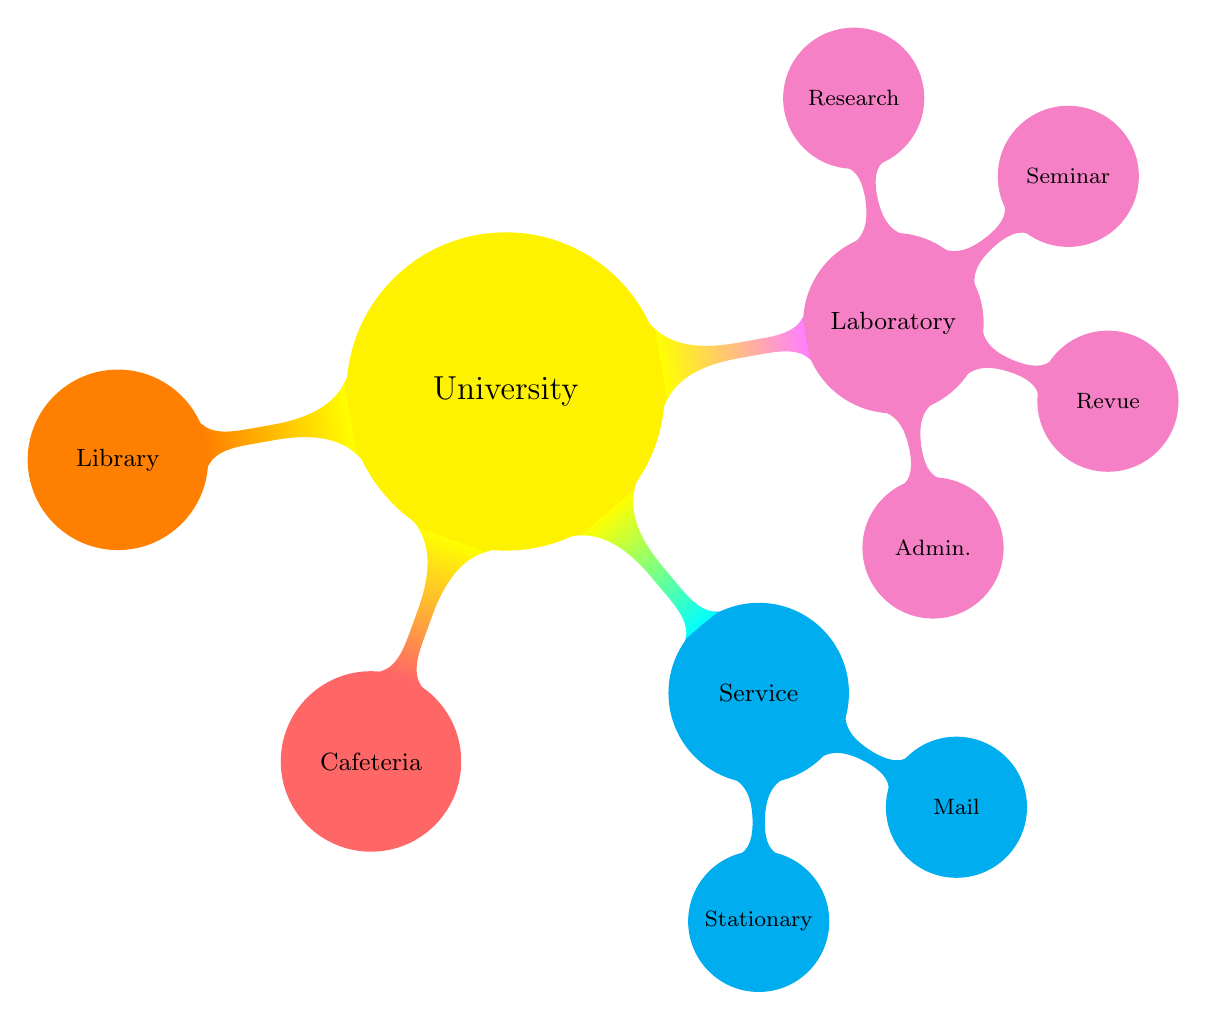
\begin{tikzpicture}
\path[mindmap,concept color=yellow,text=black]
node[concept] {University}
[clockwise from=10]
child[concept color=magenta!50!white] {
	node[concept] {Laboratory}
	[clockwise from=100]
	child { node[concept] {Research} }
	child { node[concept] {Seminar} }
	child { node[concept] {Revue} }
	child { node[concept] {Admin.} }
}  
child[concept color=cyan] {
	node[concept] {Service}
	[clockwise from=-30]
	child { node[concept] {Mail} }
	child { node[concept] {Stationary} }
}
child[concept color=red!60!white] { node[concept] {Cafeteria} }
child[concept color=orange] { node[concept] {Library}
};
\end{tikzpicture}}

\end{columns}
\end{frame}

%------------------------------------------------
\iffalse
\begin{frame}
\transfade
\frametitle{Animation with Tikz}
\scalebox{0.5}{
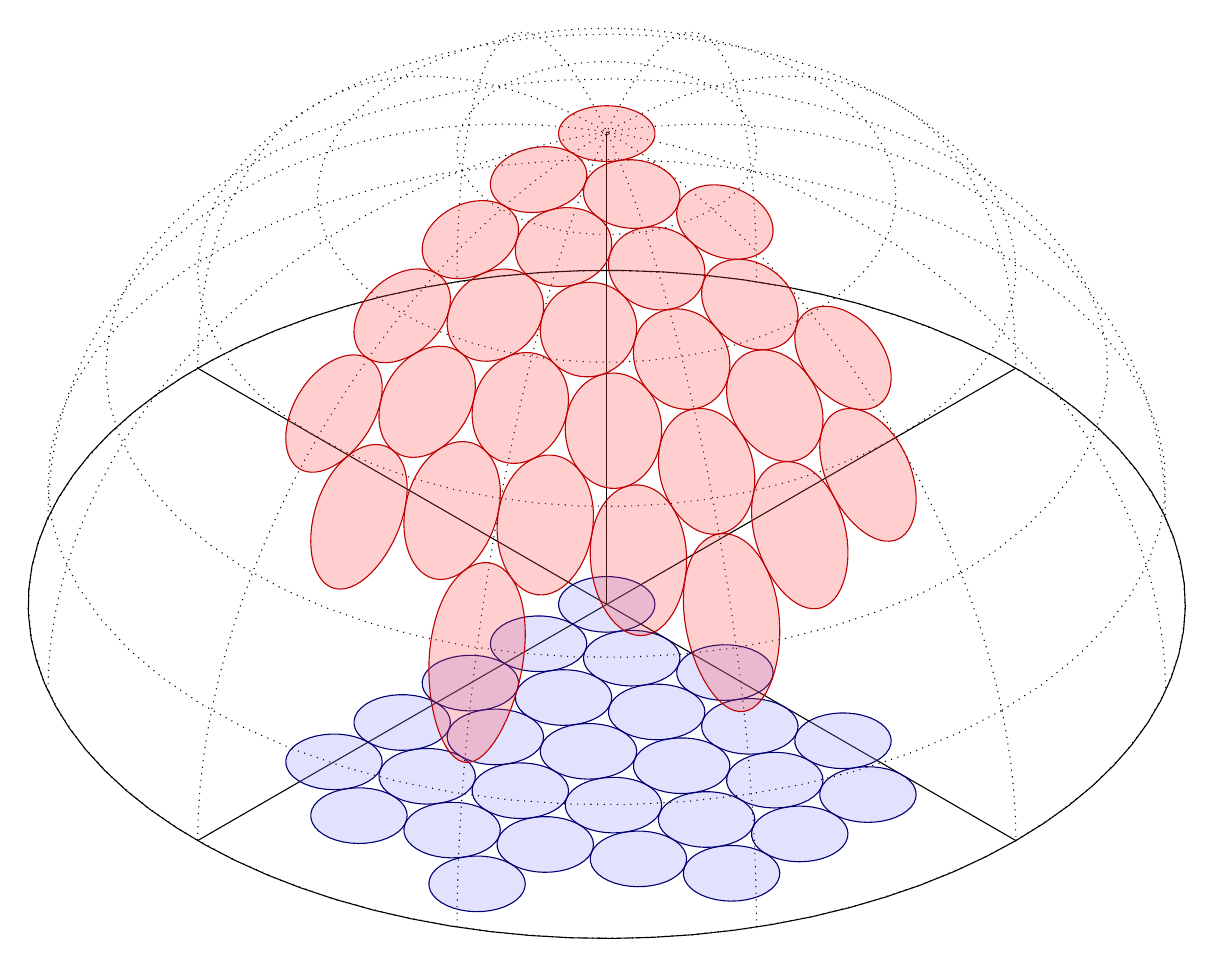
\begin{tikzpicture}[x = (-30:1cm), y = (30:1cm), z = (90:1cm)]
\def\R{6}

\begin{pgfonlayer}{dome floor}
\draw (-\R,0,0) -- (\R,0,0);
\draw (0,-\R,0) -- (0,\R,0);
\draw plot [domain = 0:360, samples = 90, variable = \i]
(\R*cos \i, \R*sin \i, 0) -- cycle;
\end{pgfonlayer}

\draw (0,0,0) -- (0,0,\R);

\begin{pgfonlayer}{dome surface}
\foreach \i in {0, 30,...,150}
\draw [dotted] plot [domain = -90:90, samples = 60, variable = \j]
(\R*cos \i*sin \j,\R*sin \i*sin \j, \R*cos \j);
\foreach \j in {0, 15,...,90}
\draw [dotted] plot [domain = 0:360, samples = 60, variable = \i]
(\R*cos \i*sin \j,\R*sin \i*sin \j, \R*cos \j);
\end{pgfonlayer}

\def\r{0.5}
\foreach \m [evaluate = {\N=max(-4, \m-7);}]in {0,...,5}{
	\foreach \n in {0,-1,...,\N}
	{\addcircle{\R}{\m*sin 60}{\n-mod(abs(\m),2)*\r}{\r}}}
\end{tikzpicture}}
\end{frame}
\fi
%------------------------------------------------
\begin{frame}[fragile]
\transfade
\centering
\frametitle{Illustration with tikz package}
\begin{columns}[c] % left column
\begin{column}{0.6\textwidth}
The \verb|tikz| package provides lots of drawing tool.

\begin{Verbatim}[fontsize=\tiny,numbers=left,frame=single,label=\LaTeX{} code]
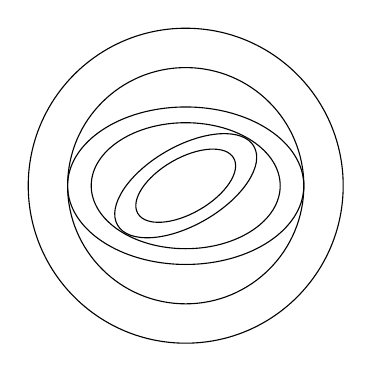
\begin{tikzpicture}[scale=1]
\draw (0,0) circle [radius=1.5];
\draw (0,0) circle (2cm); % old syntax
\draw (0,0) circle [x radius=1.5cm,y radius=10mm];
\draw (0,0) circle (1.2cm and 8mm); % old syntax
\draw (0,0) circle [x radius=1cm,
	y radius=5mm, rotate=30];
\draw[rotate=30] (0,0)
	ellipse (20pt and 10pt);  % old syntax
\end{tikzpicture}
\end{Verbatim}
Example from \textit{texample.net}
\end{column}

\begin{column}{0.4\textwidth}  \centering
\begin{figure}
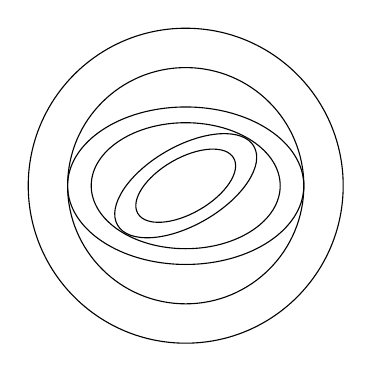
\begin{tikzpicture}[scale=1]
\draw (0,0) circle [radius=1.5];
\draw (0,0) circle (2cm); % old syntax
\draw (0,0) circle [x radius=1.5cm, y radius=10mm];
\draw (0,0) circle (1.2cm and 8mm); % old syntax
\draw (0,0) circle [x radius=1cm, y radius=5mm, rotate=30];
\draw[rotate=30] (0,0) ellipse (20pt and 10pt);  % old syntax
\end{tikzpicture}
\caption{A figure drawn entirely by \LaTeX{} code}
\end{figure}
\end{column}
\end{columns}

\end{frame}

%------------------------------------------------
\begin{frame}[fragile]
\transfade
\centering
\frametitle{Plot functions with tikz package}
\begin{columns}[c] % left column
\begin{column}{0.6\textwidth}
It's also possible to plot symbolic functions!

\begin{Verbatim}[fontsize=\tiny,numbers=left,frame=single,label=\LaTeX{} code]
\begin{tikzpicture}[domain=0:4] 
\draw[very thin,color=gray] (-0.1,-1.1)
	grid (3.9,3.9);
\draw[->] (-0.2,0) -- (4.2,0) node[right] {$x$}; 
\draw[->] (0,-1.2) -- (0,4.2) node[above] {$f(x)$};
\draw[color=red]
	plot (\x,\x})
	node[right] {$f(x) =x$}; 
\draw[color=blue]
	plot (\x,{sin(\x r)})
	node[right] {$f(x) = \sin x$}; 
\draw[color=orange]
	plot (\x,{0.05*exp(\x)})
	node[right] {$f(x) = \frac{1}{20} \mathrm e^x$};
\end{tikzpicture}
\end{Verbatim}
Example from \textit{texample.net}
\end{column}

\begin{column}{0.4\textwidth}  \centering
\scalebox{0.5}{
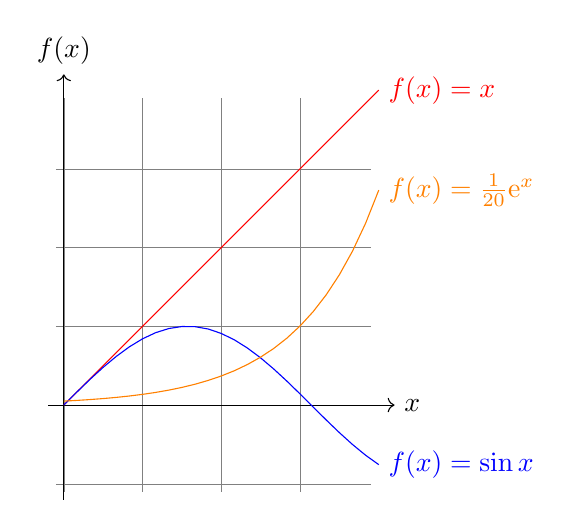
\begin{tikzpicture}[domain=0:4] 
\draw[very thin,color=gray] (-0.1,-1.1) grid (3.9,3.9);
\draw[->] (-0.2,0) -- (4.2,0) node[right] {$x$}; 
\draw[->] (0,-1.2) -- (0,4.2) node[above] {$f(x)$};
\draw[color=red]    plot (\x,{\x+0}) node[right] {$f(x) =x$}; 
\draw[color=blue]   plot (\x,{sin(\x r)})    node[right] {$f(x) = \sin x$}; 
\draw[color=orange] plot (\x,{0.05*exp(\x)}) node[right] {$f(x) = \frac{1}{20} \mathrm e^x$};
\end{tikzpicture}}
\end{column}
\end{columns}
\end{frame}

%------------------------------------------------
\begin{frame}[fragile]
\transfade
\frametitle{Animation}
We can also embed any animation using \verb|animate| package.\\~
Requirement:
\begin{itemize}
\item Adobe Acrobat Reader version 6 or above
\item A sequence of images
\end{itemize}

\begin{figure}
%\scalebox{0.5}{
%\animategraphics[loop,controls,width=\linewidth]{10}{Animations/imadethis-}{1}{131}
%}
\scalebox{0.3}{
	\animategraphics[autoplay,loop,controls,width=\linewidth]{50}{Animations/mathhien-}{0}{147}
}
\caption{(c) Bees \& Bombs}
\end{figure}
\end{frame}

%------------------------------------------------
\begin{frame}[fragile]
\transfade
When the video file is BIG $ \rightarrow $ link it to external player with \verb|href| package.\\~

\begin{Verbatim}[fontsize=\small,numbers=left,frame=single,label=\LaTeX{} code]
\href{run:Videos/video_zerog.mp4}{Click for video}
\end{Verbatim}

\begin{center}
\href{run:Videos/video_zerog.mp4}{Click for video}
\end{center}

\end{frame}

%------------------------------------------------
\subsection{Other media}

\begin{frame}[fragile]
\transfade
\frametitle{Code highlighting}
Use \verb+minted+ package to highlight code in the slide. Examples:

\begin{block}{Python}
\begin{minted}{python}
# Here is Python code
import numpy as np
for i in np.arange(6):
  print sin(i)
\end{minted}
\end{block}
\begin{block}{MATLAB}
\begin{minted}{matlab}
% Here is Matlab code
plot(x,y);
xlabel('Evolution of kinetic energy');
\end{minted}
\end{block}
\end{frame}
%------------------------------------------------ZOOM
%\begin{frame}
%\transfade
%\frametitle{Zoom to part of big image}
%\framezoom<1><2>[border](4.9cm,2.7cm)(0.5cm,0.5cm)
%\begin{figure}
%\centering
%\includegraphics[width=\textheight]{Figures/1515215.eps}
%\end{figure}
%\end{frame}

%------------------------------------------------
\begin{frame}[fragile] % Need to use the fragile option when verbatim is used in the slide
\transfade
\frametitle{Citation}
Use the \verb|\cite{key}| command to cite within the presentation (note that Beamer \textbf{does not} support BibTeX):\\~

This statement requires citation \cite{p1}.\\

Or, by copying information from .bbl file generated by BibTeX.
\end{frame}

%------------------------------------------------

\begin{frame}
\transfade
\frametitle{References}
\footnotesize{
\begin{thebibliography}{99} % Beamer does not support BibTeX so references must be inserted manually as below
\bibitem[Hien, 2016]{p1} Hien Nho Gia Nguyen (2016)
\newblock LaTeX for novices
\newblock \emph{LaSIE journal} 12(3), 45 -- 678.
\end{thebibliography}
}
\end{frame}

%------------------------------------------------
\section{Learning resources}
\begin{frame}
\transfade
\frametitle{Resources}
Some resources for \LaTeX{} self-learners:
\begin{itemize}
  \item \textbf{tex.stackexchange.com} (QA everything about \LaTeX{})
  \item \textbf{texnique.fr} (french community)
  \item \textbf{texample.net} (Examples ready for copy-paste)
  \item Editors: \textbf{texstudio.org}, \textbf{xm1math.net/texmaker}, vim + TeX plugin
  \item \textbf{detexify} (there is an android app)
  \item \textbf{Ask us! Antoine (b63), Antoine (b50), Hien (b64)}
\end{itemize}
\end{frame}
%------------------------------------------------
\begin{frame}
\transfade
\LARGE{\centerline{The End}}
\begin{center}
\small{(but, there is more to discover...)}
\end{center}
\begin{columns}[t]

\begin{column}{0.25\textwidth}
\vspace{0.3cm}
\centering
{\small Chess input}\\

\scalebox{0.3}{
\newgame
\showboard
}
\end{column}
\begin{column}{0.25\textwidth}
\centering
{\small Music input}\\
\vspace{0.3cm}
\vfill
\begin{music}
\trebleclef
\end{music}
\vfill
\end{column}

\begin{column}{0.25\textwidth}
\centering
{\small Chemistry input}\\
\vspace{0.3cm}
\scalebox{0.3}{
\chemfig{
	H_3C-[:72]{\color{blue}N}
	*5(-
	*6(-(={\color{red}O})-{\color{blue}N}(-CH_3)-(={\color{red}O})-{\color{blue}N}(-CH_3)-=)
	--{\color{blue}N}=-)}
}
\end{column}
\end{columns}
\end{frame}

%----------------------------------------------------------------------------------------

\end{document} 